\documentclass{beamer}
\usetheme{default}
\usepackage{amsmath}
\usepackage{amssymb}
\usepackage{amsthm}
\usepackage{graphicx}
\usepackage{verbatim}

% Definitions
\def\qqq{\mathbb{Q}}
\def\rrr{\mathbb{R}}
\def\zzz{\mathbb{Z}}
\def\fff{\mathbb{F}}
\def\gftwo{\mathbb{F}_2}
\def\zzzp{\mathbb{Z}_p}
\def\zzzn{\mathbb{Z}_N}
\def\zg{\mathbb{Z}_g}
\def\nnn{\mathbb{N}}
\def\BF{\mathcal{BF}}
\def\xn{(x_n)}
\def\yn{(y_n)}
\def\zn{(z_n)}
\def\an{(a_n)}
\def\Chi{\raisebox{2pt}{$\chi$}}
% \def\qed{$\Box}
% \newcounter{padic}

\begin{document}
\title{Bent Sequences and Feedback with Carry Shift Registers}
\author{Charles Celerier}
\date{SASMC 2012}
\frame{\titlepage}
%\frame{\tableofcontents}

\section{Introduction}
\subsection{What is a pseudorandom sequence?}
\begin{frame}{What is a pseudorandom sequence?}
  \begin{itemize}
      \pause
    \item[R1.] uniform distribution \[|\sum_{n=1}^p(-1)^{a_n}|\leq1\]
      \pause
    \item[R2.] \[\frac{1}{2^i}\text{ of the runs have length } i\]
      \pause
    \item[R3.] low auto-correlation, \[C(\tau)
      =\frac{\sum_{n=1}^p(-1)^{a_n+a_{n+\tau}}}{p}\]
  \end{itemize}
\end{frame}

\begin{frame}{Examples}
  \begin{example}
    \[
    a = [0,0,0,1,0,1,1]
    \]
    \begin{itemize}
        \pause
      \item[R1.] true. \[\sum_{n=1}^7(-1)^{a_n}=1\]
        \pause
      \item[R2.] true. 
        \pause
      \item[R3.] true. \[C(\tau)=\frac{\sum_{n=1}^7(-1)^{a_n+a_{n+\tau}}}{7}
        =\frac{-1}{7}\]
    \end{itemize}
  \end{example}
\end{frame}

\subsection{Stream Ciphers}
\begin{frame}{Stream Ciphers}
  \begin{tabular}{c c c c}
    \pause
              & 0101001101000001010100110100110101000011 & = & SASMC\\
              \pause
     $\oplus$ & 0001100000001011000111110001110100010010 & \\
              \hline 
              \pause
              & 0100101101001010010011000101000001010001 & = & KJLPQ
  \end{tabular}
\end{frame}

\begin{frame}{Why use stream ciphers?}
  \begin{itemize}
      \pause
    \item plaintext length is not always known
      \pause
    \item fast
      \pause
    \item easy to implement with hardware
      \pause
    \item near one-time-pad security
  \end{itemize}
\end{frame}

\begin{frame}{Topics}
  \begin{itemize}
    \item Boolean functions
    \item Feedback with Carry Shift Registers
    \item 2-adic integers
    \item Bent Sequences
  \end{itemize}
\end{frame}

\section{Boolean Functions}
\subsection{GF(2)}
\begin{frame}{$\gftwo$ or ``GF two''}
  \begin{table}[h!]\label{tab:GF(2)}
    \centering
    \begin{tabular}{|c|c|}
      \hline
      XOR&AND\\
      \hline
      $0\oplus0:=0$&$0\cdot0:=0$\\
      $0\oplus1:=1$&$0\cdot1:=0$\\
      $1\oplus0:=1$&$1\cdot0:=0$\\
      $1\oplus1:=0$&$1\cdot1:=1$\\
      \hline
    \end{tabular}
  \caption{Binary Operations for $\gftwo$}
  \end{table}
\end{frame}

\begin{frame}{$\gftwo^n$ or ``GF two to the n''}
\begin{example}
  Let $a,b\in\gftwo^3$ such that $a=(1,0,1)$ and $b=(0,1,1)$ then
  \begin{align*}
    a+b      &=(1\oplus0,0\oplus1,1\oplus1)=(1,1,0) \\
  a\cdot b &=1\cdot0\oplus0\cdot1\oplus1\cdot1=1
  \end{align*}
\end{example}

\begin{fact}
  $\gftwo^n$ is a vector space.
\end{fact}
\end{frame}

\begin{frame}{Properties of $x\in\gftwo^n$}
  \begin{definition}
  \label{def:Hamming}
  	Let $x,y\in\gftwo^n$. Then $wt:\gftwo^n\rightarrow\{0,\cdots,n\}$
    is defined by
  	\[
  	  wt(x):=\sum_{i=0}^{n-1}x_i
  	\]
  	and $d:\gftwo^n\times\gftwo^n\rightarrow\nnn\cup\{0,\cdots,n\}$
    is defined by
  	\[
  	  d(x,y):=w(x+y).
  	\]
  	Then $wt(x)$ is the {\bf Hamming\ weight} of $x$ and $d(x,y)$ is the
  	{\bf Hamming\ distance} between $x$ and $y$.
  \end{definition}
\end{frame}
  
\begin{frame}{Some examples}
  \begin{example}
  	Let $a,b,c\in\gftwo^5$ such that
  	\[
  	a=(0,1,1,0,1),\ b=(1,1,1,0,0),\ {\rm and}\ c=(0,0,1,1,0).
  	\]
  	Then,
  	\begin{center}
  		\begin{tabular}{c c}
  			$wt(a)=3$&$d(a,b)=2$\\
  			$wt(b)=3$&$d(a,c)=3$\\
  			$wt(c)=2$&$d(b,c)=3$.\\
  		\end{tabular}
  	\end{center}
  \end{example}
\end{frame}

\subsection{Boolean Functions}
\begin{frame}{Boolean functions in $\BF_n$}
  \begin{definition}
  \label{def:boolean-function}
    Any function $f$ defined such that 
    \begin{equation*}
      f:\gftwo^n\rightarrow\gftwo
    \end{equation*}
    is a {\bf Boolean function}. The set of all Boolean functions on $n$
    variables will be denoted by $\BF_n$.
  \end{definition}
\end{frame}

\begin{frame}{An example}
  \begin{example}
    Let $f=x_0+x_1$.
    \begin{table}
    \label{tab:truth-table}
    	\centering
      \begin{tabular}{|c|c||c|}
        \hline
        $x_0$&$x_1$&$f(x_0,x_1)$\\
        \hline
        0&0&0\\
        1&0&1\\
        0&1&1\\
        1&1&0\\
      	\hline
    	\end{tabular}
    	\caption{Truth Table of $f$}
    \end{table}
  \end{example}
\end{frame}

\subsection{Walsh Transform}
\begin{frame}{Characters of $\gftwo^n$}
\begin{definition}
  A {\bf character} $\Chi$ of a finite abelian group $G$ is a group
  homomorphism from $G$ into the multiplicative group of complex numbers.
\end{definition}
  \begin{fact}
    $\Chi_\lambda(x):=(-1)^{\lambda\cdot x}$ where $\lambda,x\in\gftwo^n$ is a
    {\bf group\ character} of $\gftwo^n$.
  \end{fact}
\end{frame}
\begin{frame}{Walsh Transform}
  Let the {\bf dual\ group} $\hat{\gftwo^n}$ be the group of all
  characters of $\gftwo^n$.
  \begin{itemize}
      \pause
    \item[] \[ (\Chi\cdot\psi)(x)=\Chi(x)\psi(x),\ x\in\gftwo^n  \]
      \pause
    \item[] \[\gftwo^n\cong\hat{\gftwo^n}\]
  \end{itemize}
\end{frame}

\begin{frame}{Walsh Transform}
  \begin{definition}\label{def:pBF}
    Let $f\in\BF_n$. Then $\hat{f}:\gftwo^n\rightarrow\{1,-1\}$ such that
    $\hat{f}(x)=(-1)^{f(x)}$ is a \textit{pseudo-Boolean function}
  \end{definition}
  \begin{example}
    Let $f=x_0+x_1$.
    \begin{table}
    \label{tab:truth-table}
    	\centering
      \begin{tabular}{|c|c||c|c|}
        \hline
        $x_0$&$x_1$&$f(x_0,x_1)$&$\hat{f}(x_0,x_1)$\\
        \hline
        0&0&0&1\\
        1&0&1&-1\\
        0&1&1&-1\\
        1&1&0&1\\
      	\hline
    	\end{tabular}
      \caption{Truth Table of $\hat{f}$}
    \end{table}
  \end{example}
\end{frame}

\begin{frame}{Walsh Transform}
  \begin{definition}\label{def:walsh}
    Let $f\in\BF_n$ and $\lambda\in\gftwo^n$. Then the {\em Walsh transform}
    of $f$ is defined by:
    \begin{equation}\label{eqn:walsh}
      \mathcal{W}_f(\lambda)=\sum_{x\in\gftwo^n}\hat{f}(x)\Chi_\lambda(x).
    \end{equation}
  \end{definition}
\end{frame}

\begin{frame}{Walsh Transform}
  \begin{lemma}
    The characters of $\gftwo^n$ belong to $\hat{\BF}_n
    =\{\hat{f}:f\in\BF_n\}$ and form an orthonormal basis of
    $\hat{\BF}_n\otimes\mathbb{R}$.
  \end{lemma}
  \begin{lemma}
    For $\hat{f}\in\hat{\BF}_n$,
  \begin{equation}\label{eqn:rewrite-pseudo}
  	\hat{f}(x)
      =\frac{1}{2^{n/2}}
        \sum_{\lambda\in\gftwo^n}c(\lambda)\Chi_\lambda(x)
  \end{equation}
  	where $c(\lambda)$ are given by
    \begin{equation}\label{eqn:clambda}
      c(\lambda)=\frac{1}{2^{n/2}}\mathcal{W}_f(\lambda)
    \end{equation}
  \end{lemma}
  Call the $c(\lambda)$'s {\bf Fourier coefficients}.
\end{frame}

\subsection{Bent Functions}
\begin{frame}{Rothaus' Definition and First Theorem}
  \begin{definition}\label{def:bent-function}
    If all of the Fourier coefficients of $\hat{f}$ are $\pm1$ then
    $f$ is a {\bf bent\ function}.
  \end{definition}
  \begin{theorem}\label{thm:deg-of-bent-function}
  	If $f$ is a bent function on $\gftwo^n$, then $n$ is even, $n=2k$.
    Moreover, the degree of $f$ is at most $k$, except in the case $k=1$.
  \end{theorem}
\end{frame}

\begin{frame}{Properties of Bent Functions}
  \begin{enumerate}
      \pause
    \item[(R1) 1.] $wt(f)=2^{n-1}\pm2^{n/2-1}$
      \pause
    \item[(R2) 2.] perfectly non-linear
      \pause
    \item[(R3) 3.] $\sum_{x\in\gftwo^n}{f(x)+f(x+a)}=0 \ \ \forall a\in\gftwo^n$
  \end{enumerate}
\end{frame}

\section{Feedback with Carry Shift Registers}
\subsection{Finite State Machines}
\begin{frame}{Finite State Machines}
\begin{definition}
  A {\bf finite state machine} consists of a finite collection of {\bf states}
  $K$, which sequentially accepts a sequence of {\bf inputs} from a finite set
  $A$, and produces a sequence of {\bf outputs} from a finite set
  $B$. Moreover, there is an {\bf output function} $\mu$ which computes
  the present output as a fixed function of present input and present state,
  and a
  {\bf next state function} $\delta$ which computes the next states as a fixed
  function of present input and present state. In a more mathematical manner,
  $\mu$ and $\delta$ are defined such that
  \begin{eqnarray}
    \mu:K \times A \rightarrow B \quad &\mu(k_n,a_n)=b_n \\
    \delta:K \times A \rightarrow K \quad &\delta(k_n,a_n)=k_{n+1}
  \end{eqnarray}
\end{definition}
\end{frame}
\subsection{Definition}
\begin{frame}{FCSR}
  \begin{figure}[h!]
    \centering
    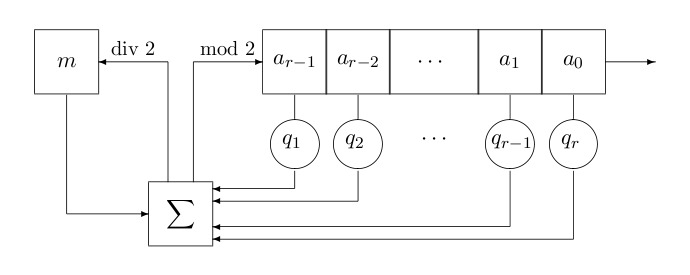
\includegraphics[totalheight=0.5\textheight]{fcsr.jpg}
    \caption{Feedback with Carry Shift Register}
  \end{figure}
\end{frame}
\begin{frame}{FCSR}
  \begin{figure}[h!]
    \centering
    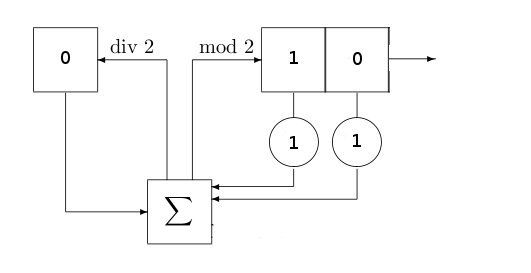
\includegraphics[totalheight=0.5\textheight]{small-fcsr-1.jpg}
  \end{figure}
\end{frame}
\begin{frame}{FCSR}
  \begin{figure}[h!]
    \centering
    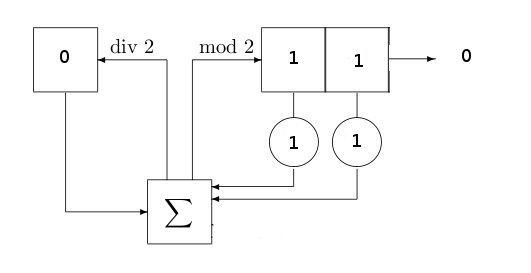
\includegraphics[totalheight=0.5\textheight]{small-fcsr-2.jpg}
  \end{figure}
\end{frame}
\begin{frame}{FCSR}
  \begin{figure}[h!]
    \centering
    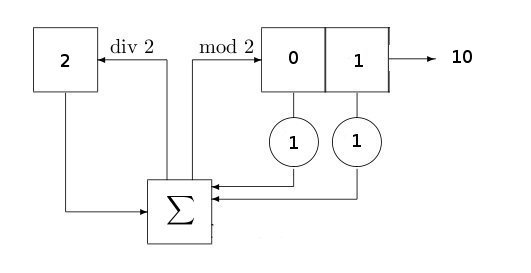
\includegraphics[totalheight=0.5\textheight]{small-fcsr-3.jpg}
  \end{figure}
\end{frame}
\begin{frame}{FCSR}
  \begin{figure}[h!]
    \centering
    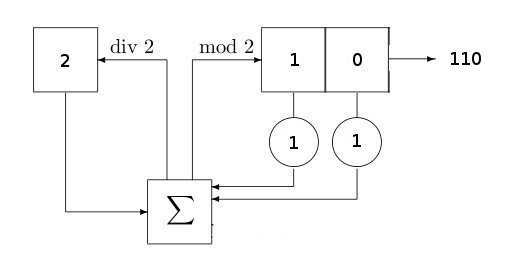
\includegraphics[totalheight=0.5\textheight]{small-fcsr-4.jpg}
  \end{figure}
\end{frame}

\subsection{Breaking a Stream Cipher}
\begin{frame}{Breaking a Stream Cipher}
  \textit{Kerckhoffs' principle}: ``In assessing the security of a
  cryptosystem, one should always assume the enemy knows the method being
  used.''\\
  \ \\
  Typically, breaking a stream cipher will mean recovering the state of
  the shift register at a given time.
\end{frame}

\section{Pseudorandom Sequences of 0s and 1s}
\subsection{Analyzing}
\begin{frame}{Two Methods}
  \begin{enumerate}[1.]
      \pause
    \item 2-adic integers
      \pause
    \item Boolean sequences
  \end{enumerate}
\end{frame}

\section{2-adic integers}
\begin{frame}{2-adic integers}
  What happens when we write positive integers with infinitely many digits? \\
  \pause
  \begin{definition}
    The infinite integer sequence $\xn$
    determines a {\bf 2-adic integer} $\alpha$, or
    $\xn \rightarrow \alpha$, if
    \begin{equation} \label{eq:seq}
    x_{i+1} \equiv x_i\pmod{2^{i+1}} \ \ \ \forall i \geq 0.
    \end{equation}
    Two sequences $\xn$ and $(x_n')$ determine the same $2$-adic integer if 
  \begin{equation} \label{eq:equiv}
    x_i \equiv x_i' \pmod{2^{i+1}}\ \ \ \forall i \geq 0.
  \end{equation}
    The {\bf set of all 2-adic integers} will be denoted by $\zzz_2$.
  \end{definition}
\end{frame}

\begin{frame}{2-adic integers}
\begin{example} \label{ex:equiv-seq}
  Let $\xn \rightarrow \alpha \in \zzz_2$. Then the first 5 terms of
  $\xn$ may look something like:
  \begin{align*}
    \xn = (&\ 1\ , \ 1+1\cdot2 \ , \ 1+1\cdot2+0\cdot2^2 \ ,\\
            &1+1\cdot2+0\cdot2^2+0\cdot2^3 \ ,
            \ 1+1\cdot2+0\cdot2^2+1\cdot2^4 \ ,
              \ \dots)\\
        = (&1,3,3,3,19,\dots)
  \end{align*}
  Then an equivalent sequence to $\xn$ could look entirely different:
  \begin{align*}
    \yn &= (19,3,3,19,19,\dots) \\
  \end{align*}
\end{example}
\end{frame}

\begin{frame}{2-adic integers}
  \begin{align*}
    \alpha&=11001\cdots\\
    1&=1000\cdots\\
    2&=0100\cdots\\
    3&=1100\cdots\\
    -1&=1111\cdots\\
    1/3&=1101010101\cdots\\
    -1/3&=1010101010\cdots
  \end{align*}
\end{frame}

\begin{frame}{2-adic integers}
  \begin{definition}
    Let $\alpha=\an\in\zzz_2\setminus(0)$. If $m$ is the smallest number in
    $\nnn\cup\{0\}$ such that $a_m \not\equiv 0 \pmod 2^{m+1}$, then the {\bf
    2-adic\ valuation} of $\alpha$ is $m$, or $\log_2(\alpha)=m$. If $\alpha=0$,
    then $\log_2(\alpha)=\infty$.
  \end{definition}
  \begin{example}
    Let $\alpha=0001011101111\cdots$. Then $\log_2(\alpha)=3$.
  \end{example}
\end{frame}

\section{Boolean Sequence}
\begin{frame}{Boolean Sequence}
  \pause
  \begin{definition}
    Let $(a_n)$ be a sequence. If $T$ is the smallest integer such that
    $a_i=a_{i+T}$, then the {\bf minimal\ period} of $(a_n)$ is $T$.
  \end{definition}
  
  \begin{definition}\label{def:lex-Bool-seq}
    Let $f\in\BF_n$ and $v_i\in\gftwo^n$ such that $v_i=B^{-1}(i)$ for
    $0\leq i<2^n$. Then,
    \begin{equation}
      seq(f)=(f(v_0),f(v_1),\cdots,f(v_{2^n-1}),f(v_0),\cdots)
    \end{equation}
    is a {\bf lexicographical\ Boolean\ sequence}.
  \end{definition}
  \begin{theorem}
    The lexicographical Boolean sequence of a Bent function has a period
    exactly $2^n$.
  \end{theorem}
\end{frame}

\begin{frame}{Boolean Sequence}
  \begin{definition}\label{2-adic-ex}
    Let $f\in\BF_n$ and $v_i\in\gftwo^n$ such that $v_i=B^{-1}(i)$ for
    $0\leq i<2^n$. Then,
    \begin{equation}
      \alpha_f=(f(v_0),f(v_0)+f(v_1)\cdot2,\cdots,\allowbreak
        f(v_0)+\cdots\allowbreak+f(v_i)\cdot2^i,\allowbreak\cdots)
    \end{equation}
    where $\alpha_f\in\zzz_2$ is called the {\bf 2-adic\ expansion} of $f$.
  \end{definition}
  
  \begin{lemma}
    The digit representation of $\alpha_f$ is $seq(f)$.
  \end{lemma}
\end{frame}

\subsection{Constructing}
\begin{frame}{Maiorana-McFarland Class Boolean Functions}
  \par A simple bent function construction is accomplished by the Boolean
  functions in the {\bf Maiorana-McFarland\ class}. This is the the set
  $\mathcal{M}$ which contains all Boolean functions on
  $\gftwo^n=\{(x,y):x,y\in\gftwo^{n/2}\}$, of the form:
    \[
    f(x,y)=x\cdot\pi(y)\oplus g(y)
    \]
  where $\pi$ is any permutation on $\gftwo^{n/2}$ and $g$ any Boolean
  function on $\gftwo^{n/2}$.\\
  
  \par All functions in the Maiorana-McFarland class of Boolean functions are
  bent.
\end{frame}
  
\begin{frame}
  \par Consider the subset of Maiorana-McFarland class Boolean functions where
  $g(y)=0$. $\bar{\pi}$ will be the function which specifies where each
  index moves to under the permutation $\pi$.
  
  \begin{theorem}
    $\log_2(\alpha_{x\cdot\pi(y)})=2^{n/2}+2^{\bar{\pi}(y_0)}$
  \end{theorem}

  \par The 2-adic valuation of the Boolean sequence of the functions in this
  subset is entirely dependent on the permutation $\pi$.
\end{frame}

\section{Conclusion}
\begin{frame}{Conclusion}
  \begin{itemize}
    \item Pseudorandom sequences
    \item Stream Ciphers
    \item Shift Registers
    \item Analysis using Boolean functions and 2-adic integers
    \item Connections between Bent functions and 2-adic valuation
  \end{itemize}
\end{frame}

\end{document}
